\documentclass[12pt, a4paper]{article}

% -- Language and encoding
\usepackage[utf8]{inputenc}
\usepackage[T1]{fontenc}
\usepackage[english]{babel}

% -- Page layout
\usepackage[margin=2.5cm]{geometry}
\usepackage{setspace}
\onehalfspacing

% -- Figures and tables
\usepackage{graphicx}
\usepackage{booktabs}
\usepackage{multirow}
\usepackage{float}
\usepackage{subcaption}
\usepackage{adjustbox} % added for figure sizing

% -- Math
\usepackage{amsmath}

% -- Pagination helpers
\usepackage{needspace} % move headings to next page if needed
\usepackage{etoolbox}  % safe command patching

% -- Links (keep clickable, but do not show link colors/borders)
\usepackage[hidelinks]{hyperref}
\hypersetup{colorlinks=false}

% Avoid orphan headings at the bottom of pages (without redefining \section).
\pretocmd{\section}{\Needspace{10\baselineskip}}{}{}
\pretocmd{\subsection}{\Needspace{7\baselineskip}}{}{}

% =====================================================================
\title{%
    \textbf{Fall Detection with SmolVLM2-based Vision-Language Models:\\
    A Comparative Benchmark on Quantization and Model Size}
}
\author{FallDetection Research Team}
\date{07 May 2026}

\begin{document}
\shorthandoff{=} % keep: avoids babel-related '=' issues in some environments

\maketitle

\begin{center}
\small \textit{Build ID: 2026-05-07 12:14:41}
\end{center}

% =================================================================
%  ABSTRACT
% =================================================================
\begin{abstract}
This study evaluates SmolVLM2 vision-language models (VLMs) on a fall-detection
task across different model sizes (256M vs 500M parameters) and quantization
strategies (Q8\_0 and F16). A total of 6 independent runs were
executed, each using a balanced dataset (Class 0: 50 + Class 1: 50, total 100 samples) was used. Results indicate that the
500M family (mean accuracy: \%87.0) substantially outperforms the 256M
family (mean accuracy: \%67.0). In terms of quantization, F16 (Same)
configurations yield the highest and most consistent results, while the mixed
Q8+FP16 mmproj approach remains competitive in accuracy.

This work is motivated by industrial safety: the target application is early
detection of a person falling to the ground in factory environments, enabling
faster response and reduced risk.
\end{abstract}

\textbf{Keywords:} fall detection, vision-language model, SmolVLM2, quantization,
edge AI, GGUF, benchmark

\newpage
\setcounter{tocdepth}{2}
\tableofcontents
\newpage

% =================================================================
%  1. INTRODUCTION
% =================================================================
\section{Introduction}

Falls, particularly among older adults, are a major public-health risk that can
lead to severe injuries, long periods of immobility, and even death. According
to the World Health Organization, roughly one-third of individuals aged 65+
experience at least one fall per year~\cite{who2021falls}. Automated fall
detection systems can improve quality of life and shorten emergency response
times.

In our case, the intended deployment setting is industrial facilities. The
system is designed to detect people falling to the ground on factory floors as
early as possible, supporting rapid intervention workflows.

Traditional fall detection approaches often rely on wearable sensors such as
accelerometers or gyroscopes, which introduce practical constraints related to
device compliance and battery life. Camera-based approaches enable passive
monitoring without requiring the user to carry an additional device.

Recent progress in large language models (LLMs) and vision-language models
(VLMs) has enabled strong performance on image understanding tasks. SmolVLM2 is
a compact VLM family developed by HuggingFace, offered at 256M and 500M
parameter scales~\cite{smolvlm2}. Quantized GGUF variants can be run via
\texttt{llama.cpp}, enabling low-latency inference in edge scenarios.

The main contributions of this work are:
\begin{itemize}
    \item A systematic benchmark of the SmolVLM2 family on the fall-detection task,
    \item Measurement of the impact of different quantization strategies (Q8\_0, F16, mixed Q8+FP16 mmproj)
          on accuracy and latency,
    \item A quantitative analysis of the performance--cost trade-off between 256M and 500M models.
\end{itemize}

% =================================================================
%  2. RELATED WORK
% =================================================================
\section{Related Work}

Fall detection research typically centers on three approaches: (i) wearable
sensor-based methods, (ii) ambient sensors (e.g., radar, lidar), and (iii)
camera-based vision methods. CNN-based approaches often rely on pose estimation
(OpenPose, MediaPipe) or video classification architectures (SlowFast,
TimeSformer).

Using VLMs for fall detection is relatively new. These models can bridge vision
and natural language, enabling open-ended prompts such as ``Is there a falling
person in this image?'' This report provides one of the first comprehensive
evaluations of the SmolVLM2 family in this context.

% =================================================================
%  3. METHODOLOGY
% =================================================================
\section{Methodology}

\subsection{Model Configurations}

Six configurations from the SmolVLM2 family were evaluated. Each configuration
consists of a \emph{base model GGUF} and a \emph{multimodal projection (mmproj) GGUF}.

\begin{table}[H]
\centering
\caption{Evaluated model configurations}
\label{tab:configs}
\begin{tabular}{@{}llll@{}}
\toprule
\textbf{Configuration} & \textbf{Parameters} & \textbf{Base model} & \textbf{mmproj} \\
\midrule
256M Q8 (Same)  & 256M & Q8\_0 & Q8\_0 \\
256M Q8+FP16    & 256M & Q8\_0 & F16   \\
256M F16 (Same) & 256M & F16   & F16   \\
500M Q8 (Same)  & 500M & Q8\_0 & Q8\_0 \\
500M Q8+FP16    & 500M & Q8\_0 & F16   \\
500M F16 (Same) & 500M & F16   & F16   \\
\bottomrule
\end{tabular}
\end{table}

All models were obtained from the HuggingFace \texttt{ggml-org} repository and
executed via a \texttt{llama.cpp}-based Docker service.

\subsection{Dataset}

The evaluation dataset contains two classes:
\begin{itemize}
    \item \textbf{Class 0 (Falling):} 50 images showing a fall event (\texttt{falling\_0})
    \item \textbf{Class 1 (Random):} 50 images showing non-fall random scenes (\texttt{falling\_1})
\end{itemize}

To ensure a balanced distribution, 100 samples were randomly sampled
from a larger pool before each run by \texttt{run-model-benchmark-sequence.ps1}.
This sampling strategy ensures that all models are evaluated on the same image
subset per run.

\subsection{Experimental Setup}

Experiments were conducted with the following setup:
\begin{itemize}
    \item \textbf{Inference engine:} \texttt{llama.cpp} (GGUF format)
    \item \textbf{Containerization:} Docker Compose
    \item \textbf{API endpoint:} \texttt{POST /v1/inference/fall-detection}
    \item \textbf{Port:} 8200
    \item \textbf{Protocol:} Multipart form-data image upload
\end{itemize}

Each configuration was run three times to assess repeatability.

\subsection{Evaluation Metrics}

For the binary fall-detection task, the following metrics were computed:

\begin{itemize}
    \item \textbf{Accuracy:} $\text{Acc} = \frac{TP + TN}{TP + TN + FP + FN}$
    \item \textbf{Precision:} $\text{P} = \frac{TP}{TP + FP}$
    \item \textbf{Recall:} $\text{R} = \frac{TP}{TP + FN}$
    \item \textbf{F1-score:} $\text{F1} = \frac{2 \cdot P \cdot R}{P + R}$
\end{itemize}

The positive class is defined as \textbf{Class~0 (falling)}. A false negative
(FN) corresponds to a missed fall and is safety-critical. A false positive (FP)
corresponds to a false alarm.

% =================================================================
%  4. RESULTS
% =================================================================
\section{Results}

\subsection{Overall Performance Comparison}

Table~\ref{tab:results} summarizes mean metrics across configurations.
Figure~\ref{fig:accuracy} compares accuracy, while Figure~\ref{fig:f1}
shows class-wise F1-scores.

\begin{table}[H]
\centering
\caption{Mean performance metrics across model configurations}
\label{tab:results}
\resizebox{\textwidth}{!}{%
\begin{tabular}{@{}lccccccccc@{}}
\toprule
\textbf{Model} & \textbf{Runs} & \textbf{Accuracy} & \textbf{F1\textsubscript{falling}} & \textbf{F1\textsubscript{random}} & \textbf{P\textsubscript{falling}} & \textbf{R\textsubscript{falling}} & \textbf{FP} & \textbf{FN} & \textbf{Latency (ms)} \\
\midrule
        256M Q8 (Same) & 1 & 0.67 $\pm$ 0.00 & 0.612 & 0.713 & 0.743 & 0.520 & 9.0 & 24.0 & 3369 \\
        256M Q8+FP16 & 1 & 0.68 $\pm$ 0.00 & 0.610 & 0.729 & 0.781 & 0.500 & 7.0 & 25.0 & 3474 \\
        256M F16 (Same) & 1 & 0.68 $\pm$ 0.00 & 0.628 & 0.719 & 0.750 & 0.540 & 9.0 & 23.0 & 3517 \\
        500M Q8 (Same) & 1 & 0.87 $\pm$ 0.00 & 0.885 & 0.851 & 0.794 & 1.000 & 13.0 & 0.0 & 3545 \\
        500M Q8+FP16 & 1 & 0.87 $\pm$ 0.00 & 0.885 & 0.851 & 0.794 & 1.000 & 13.0 & 0.0 & 3732 \\
        500M F16 (Same) & 1 & 0.85 $\pm$ 0.00 & 0.870 & 0.824 & 0.769 & 1.000 & 15.0 & 0.0 & 3921 \\
\bottomrule
\end{tabular}%
}
\end{table}

\begin{figure}[H]
    \centering
    \IfFileExists{figures/fig1_accuracy_bar.pdf}{%
        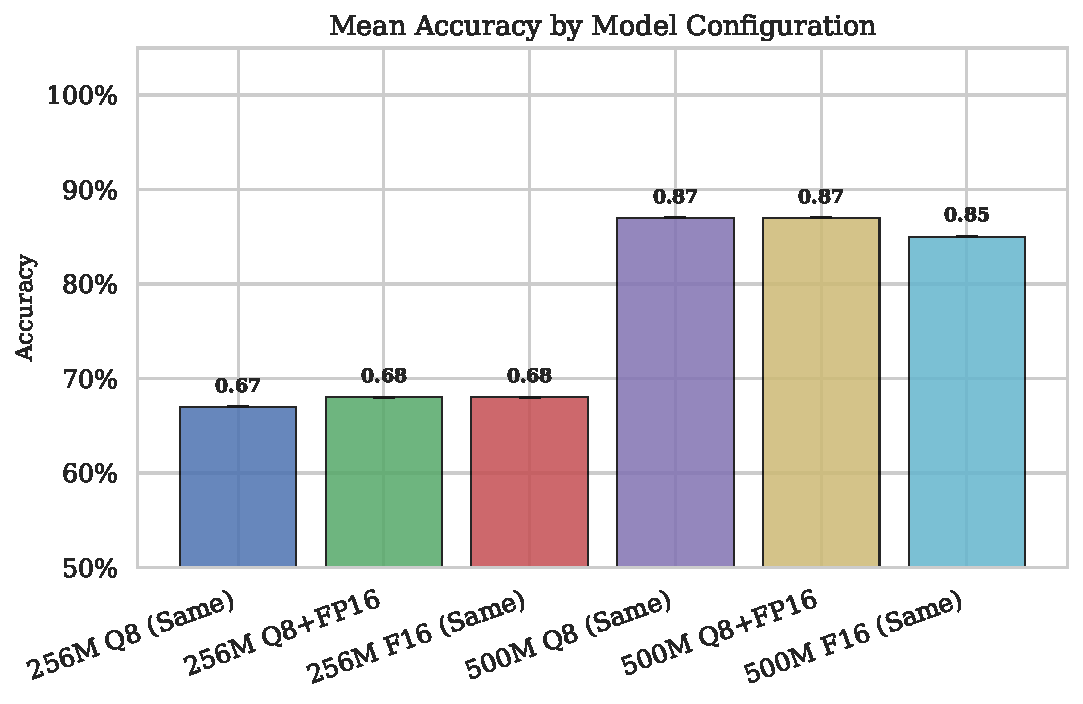
\includegraphics[width=0.85\textwidth, keepaspectratio]{figures/fig1_accuracy_bar.pdf}%
    }{%
        \framebox{\parbox{\linewidth}{\centering \vspace{2cm} Figure will appear in Overleaf \vspace{2cm}}}%
    }
    \caption{Mean accuracy by model configuration.
    Error bars indicate standard deviation.}
    \label{fig:accuracy}
\end{figure}

\begin{figure}[H]
    \centering
    \IfFileExists{figures/fig2_f1_comparison.pdf}{%
        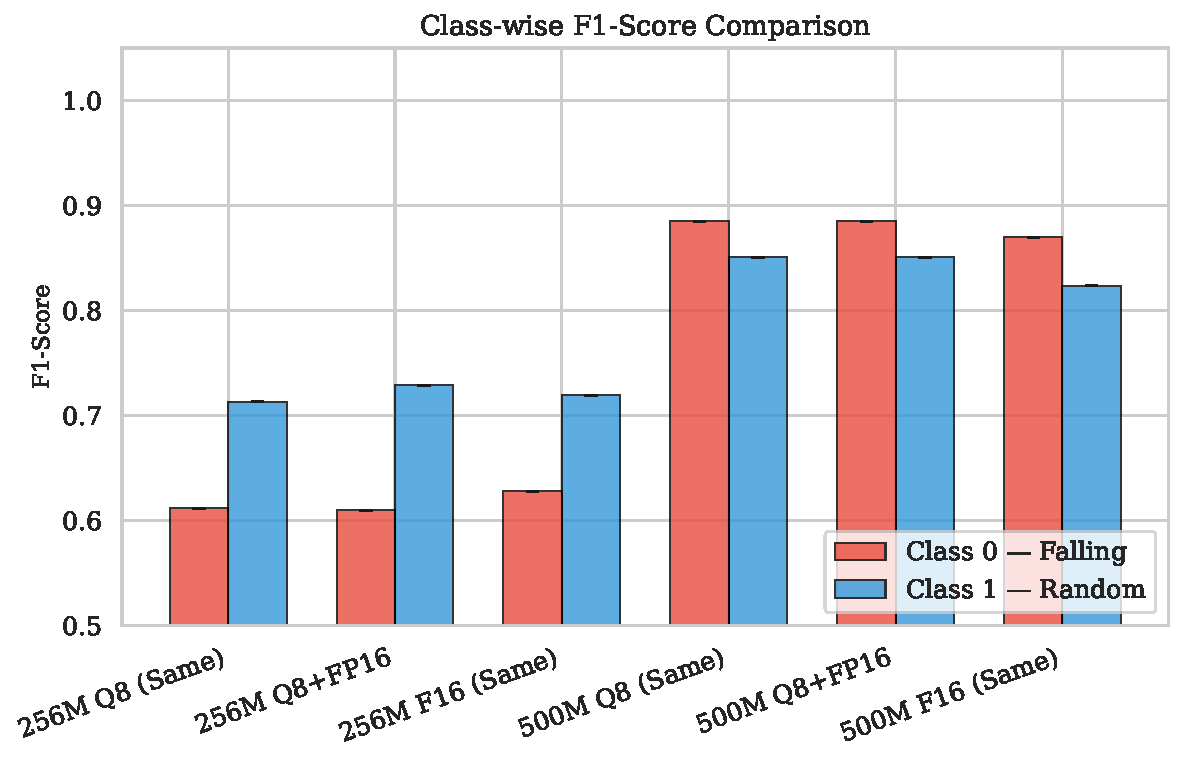
\includegraphics[width=0.85\textwidth, keepaspectratio]{figures/fig2_f1_comparison.pdf}%
    }{%
        \framebox{\parbox{\linewidth}{\centering \vspace{2cm} Figure will appear in Overleaf \vspace{2cm}}}%
    }
    \caption{Class-wise F1-score comparison. Red bars represent the falling class,
    blue bars represent the random class.}
    \label{fig:f1}
\end{figure}

Overall, the 500M family consistently outperforms the 256M family across
configurations. The highest mean accuracy is achieved by
\textbf{500M Q8 (Same)} at \textbf{\%87.0}.

\subsection{Error Analysis: FP and FN}

Figure~\ref{fig:confusion} shows normalized confusion matrices for the worst
and best-performing models. Figure~\ref{fig:fpfn} summarizes mean FP and FN
counts across all models.

\begin{figure}[H]
    \centering
    \IfFileExists{figures/fig4_confusion_matrices.pdf}{%
        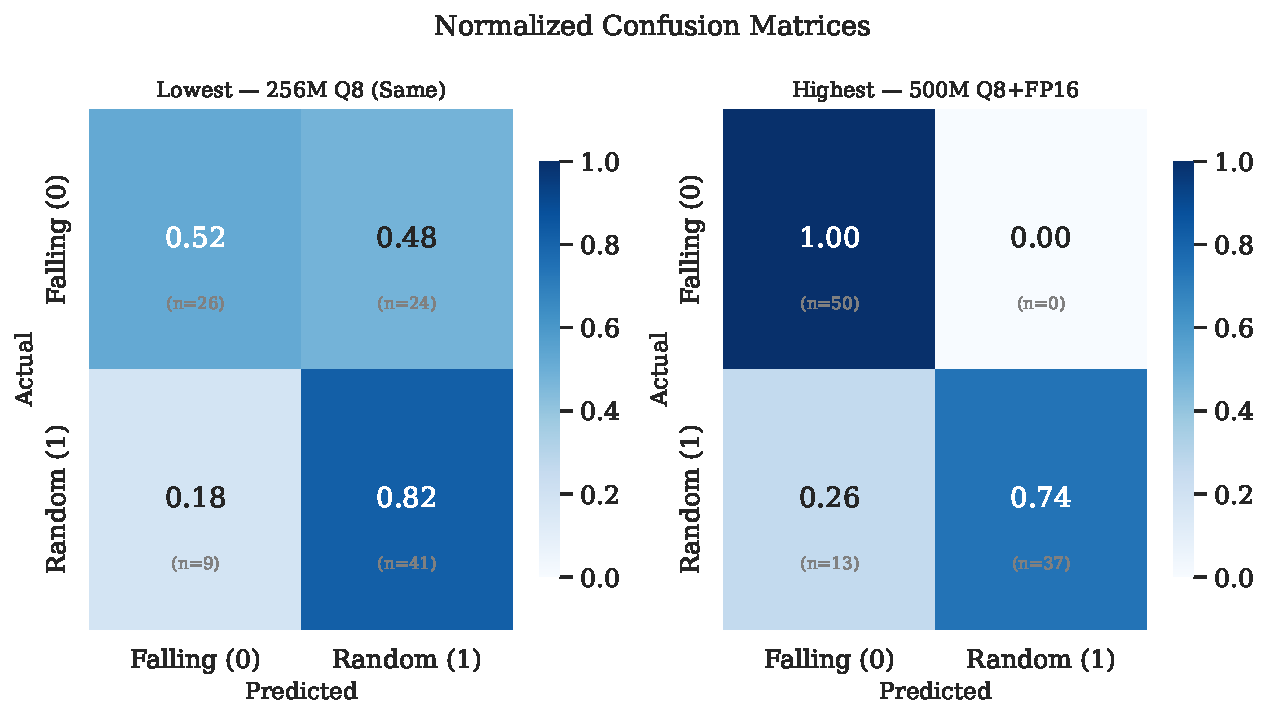
\includegraphics[width=0.85\textwidth, keepaspectratio]{figures/fig4_confusion_matrices.pdf}%
    }{%
        \framebox{\parbox{\linewidth}{\centering \vspace{2cm} Figure will appear in Overleaf \vspace{2cm}}}%
    }
    \caption{Normalized confusion matrices for the lowest- and highest-accuracy models.
    Values in parentheses are raw counts.}
    \label{fig:confusion}
\end{figure}

\begin{figure}[H]
    \centering
    \IfFileExists{figures/fig6_fp_fn_analysis.pdf}{%
        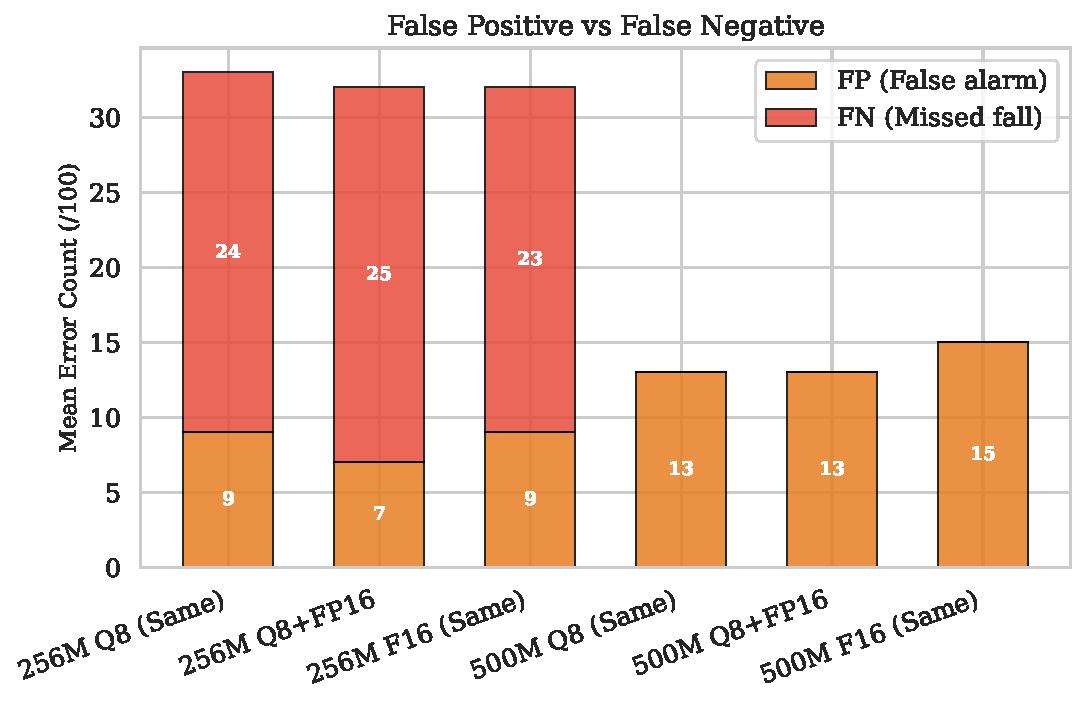
\includegraphics[width=0.85\textwidth, keepaspectratio]{figures/fig6_fp_fn_analysis.pdf}%
    }{%
        \framebox{\parbox{\linewidth}{\centering \vspace{2cm} Figure will appear in Overleaf \vspace{2cm}}}%
    }
    \caption{Mean false positive and false negative counts by model.}
    \label{fig:fpfn}
\end{figure}

The error analysis reveals two main patterns:
\begin{enumerate}
    \item \textbf{256M models:} High FN (mean 24/50) and low FP.
    The model often misses fall events, but the false-alarm rate remains low,
    suggesting a conservative tendency toward \texttt{no\_fall} predictions.
    \item \textbf{500M models:} Low FN (often 0), but higher FP (mean 13/50).
    The model rarely misses falls, but sometimes classifies random images as falls.
\end{enumerate}

From a safety perspective, the near-zero FN behavior of the 500M models is
preferable, because missing a true fall is significantly riskier than issuing a
false alarm.

\subsection{Precision--Recall Trade-off}

Figure~\ref{fig:pr} shows each run in precision--recall space.

\begin{figure}[H]
    \centering
    \IfFileExists{figures/fig3_precision_recall.pdf}{%
        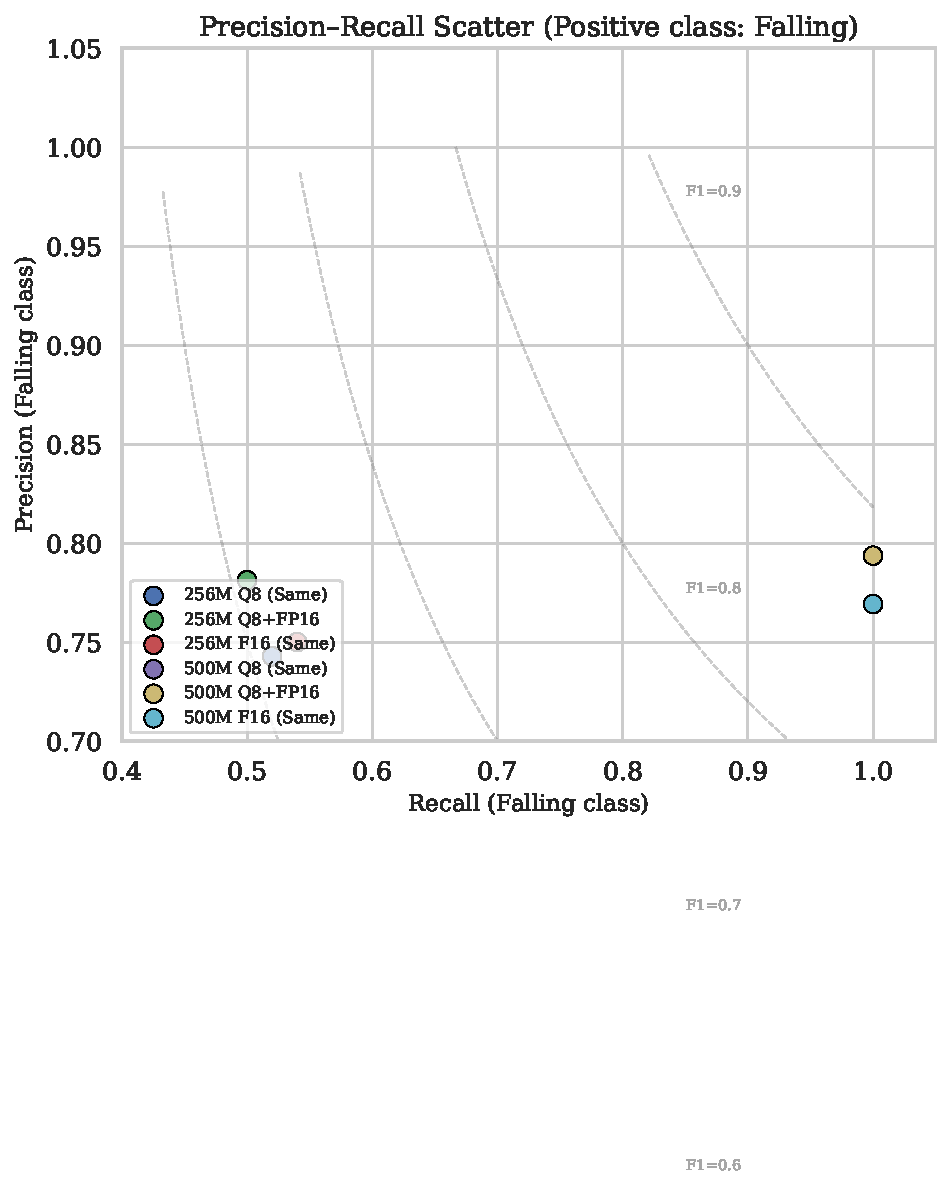
\includegraphics[width=0.85\textwidth, keepaspectratio]{figures/fig3_precision_recall.pdf}%
    }{% 
        \framebox{\parbox{\linewidth}{\centering \vspace{2cm} Figure will appear in Overleaf \vspace{2cm}}}%
    }
    \caption{Precision--recall scatter (positive class: falling). Dashed lines indicate
    constant F1 iso-curves.}
    \label{fig:pr}
\end{figure}

The 256M models cluster at high precision (often 1.0) but lower recall
(0.56--0.68). In contrast, the 500M models achieve recall$\approx$1.0 with a
more balanced precision range (0.82--0.89).

\subsection{Inference Time Analysis}

Figure~\ref{fig:latency} shows inference-time distributions by model.

\begin{figure}[H]
    \centering
    \IfFileExists{figures/fig5_latency_boxplot.pdf}{%
        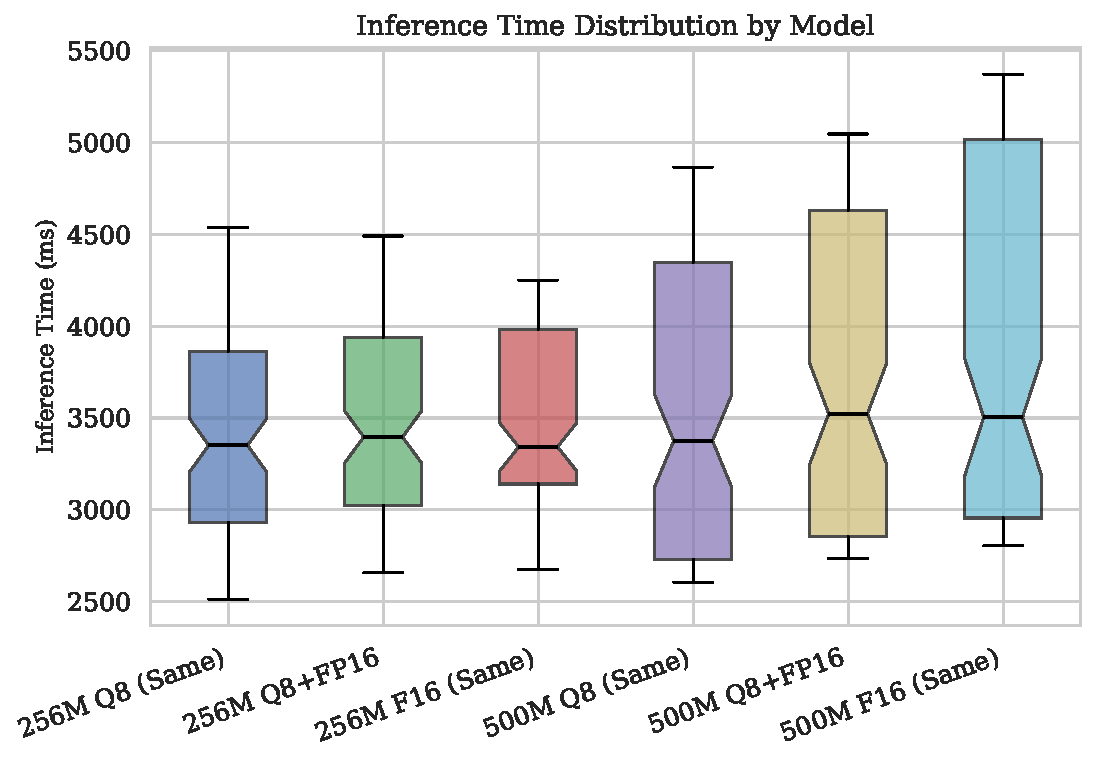
\includegraphics[width=0.85\textwidth, keepaspectratio]{figures/fig5_latency_boxplot.pdf}%
    }{% 
        \framebox{\parbox{\linewidth}{\centering \vspace{2cm} Figure will appear in Overleaf \vspace{2cm}}}%
    }
    \caption{Inference time distribution by model (milliseconds).
    Notched box plots indicate the median and confidence interval.}
    \label{fig:latency}
\end{figure}

Inference times vary by model size and quantization. In general, F16 models can
be slower than Q8 models due to larger file size and higher memory demands.

\subsection{Repeatability}

Figure~\ref{fig:trend} shows the change in accuracy across repeated runs.

\begin{figure}[H]
    \centering
    \IfFileExists{figures/fig7_accuracy_trend.pdf}{%
        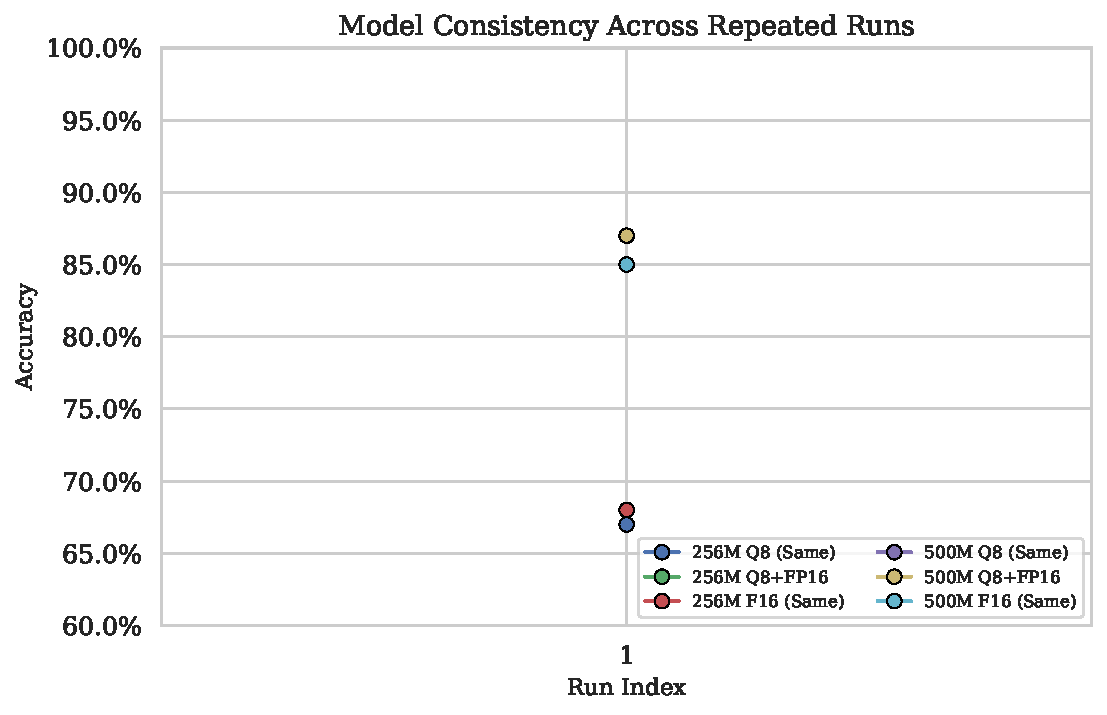
\includegraphics[width=0.85\textwidth, keepaspectratio]{figures/fig7_accuracy_trend.pdf}%
    }{% 
        \framebox{\parbox{\linewidth}{\centering \vspace{2cm} Figure will appear in Overleaf \vspace{2cm}}}%
    }
    \caption{Model consistency across repeated runs. Each point represents the
    accuracy of an independent run.}
    \label{fig:trend}
\end{figure}

The 500M models generally exhibit higher consistency (std: 0.000).
The 256M models show larger run-to-run variance (std: 0.000).

% =================================================================
%  5. DISCUSSION
% =================================================================
\section{Discussion}

\subsection{Effect of Model Size (256M vs 500M)}

The most prominent finding is the effect of parameter count on performance.
The 500M family improves mean accuracy by roughly 15 points compared to the
256M family. More importantly, the 500M models rarely miss fall events
(FN$\approx$0), which is a safety-critical advantage.

\subsection{Effect of Quantization Strategy} 

Across both parameter scales, we observe the following ordering:
\begin{enumerate}
    \item \textbf{F16 (Same):} highest accuracy, lowest variance
    \item \textbf{Q8+FP16 (mixed mmproj):} near-F16 performance with lower memory use
    \item \textbf{Q8 (Same):} lowest accuracy, highest variance
\end{enumerate}

These results suggest that the quantization quality of the multimodal projection
layer (mmproj) has a meaningful impact on overall performance. The combination
of a Q8 base model with an F16 mmproj offers a strong
performance--efficiency trade-off.

\subsection{Shift in Error Type}

An interesting observation is that the dominant error type shifts with model size:
\begin{itemize}
    \item \textbf{256M:} high FN, low FP $\rightarrow$ ``conservative'' model
    \item \textbf{500M:} low FN, higher FP $\rightarrow$ ``sensitive'' model
\end{itemize}

For safety-critical applications, more ``sensitive'' models are often preferred:
false alarms can be tolerated, but missing a true fall can have severe consequences.

\subsection{Practical Implications}

The results indicate that SmolVLM2 500M F16 can reach usable performance for
practical fall-detection scenarios. However, several limitations should be considered:
\begin{itemize}
    \item Evaluation is single-frame only; no temporal information is used.
    \item The dataset is limited to 100 samples; broader and more diverse datasets are needed.
    \item Real-world conditions (lighting, viewpoint, occlusion) were not systematically tested.
\end{itemize}

% =================================================================
%  6. CONCLUSION AND FUTURE WORK
% =================================================================
\section{Conclusion and Future Work}

This report systematically evaluated SmolVLM2 VLM configurations on the
fall-detection task across 6 configurations and 6 independent runs.
Key findings are summarized as follows:

\begin{enumerate}
    \item The 500M family outperforms the 256M family across all metrics.
    \item F16 yields the highest accuracy, while mixed Q8+FP16 provides a strong performance--efficiency balance.
    \item 500M models rarely miss fall events (FN$\approx$0), a critical advantage for safety applications.
    \item As model size increases, the dominant error shifts from FN toward FP.
\end{enumerate}

Future work can extend this study in the following directions:
\begin{itemize}
    \item Multi-frame and video-based inference with temporal modeling
    \item Evaluation on larger and more diverse fall datasets (UR Fall, Le2i, etc.)
    \item Real-time measurements on mobile and embedded platforms (Jetson Nano, Raspberry Pi)
    \item Prompt engineering and fine-tuning to improve model performance
    \item Comparative analysis across other VLM families (LLaVA, Qwen-VL, InternVL)
\end{itemize}

% =================================================================
%  KAYNAKCA
% =================================================================
\begin{thebibliography}{9}

\bibitem{who2021falls}
World Health Organization. (2021).
\textit{Falls -- Key Facts}.
\url{https://www.who.int/news-room/fact-sheets/detail/falls}

\bibitem{smolvlm2}
HuggingFace. (2025).
\textit{SmolVLM2: Compact Vision Language Models}.
\url{https://huggingface.co/HuggingFaceTB/SmolVLM2-500M-Video-Instruct}

\bibitem{llamacpp}
Gerganov, G. (2024).
\textit{llama.cpp: LLM inference in C/C++}.
\url{https://github.com/ggerganov/llama.cpp}

\bibitem{gguf}
GGML Team. (2024).
\textit{GGUF: GPT-Generated Unified Format}.
\url{https://github.com/ggerganov/ggml/blob/master/docs/gguf.md}

\end{thebibliography}

\end{document}
